% Created by tikzDevice version 0.10.1 on 2016-06-03 22:53:07
% !TEX encoding = UTF-8 Unicode
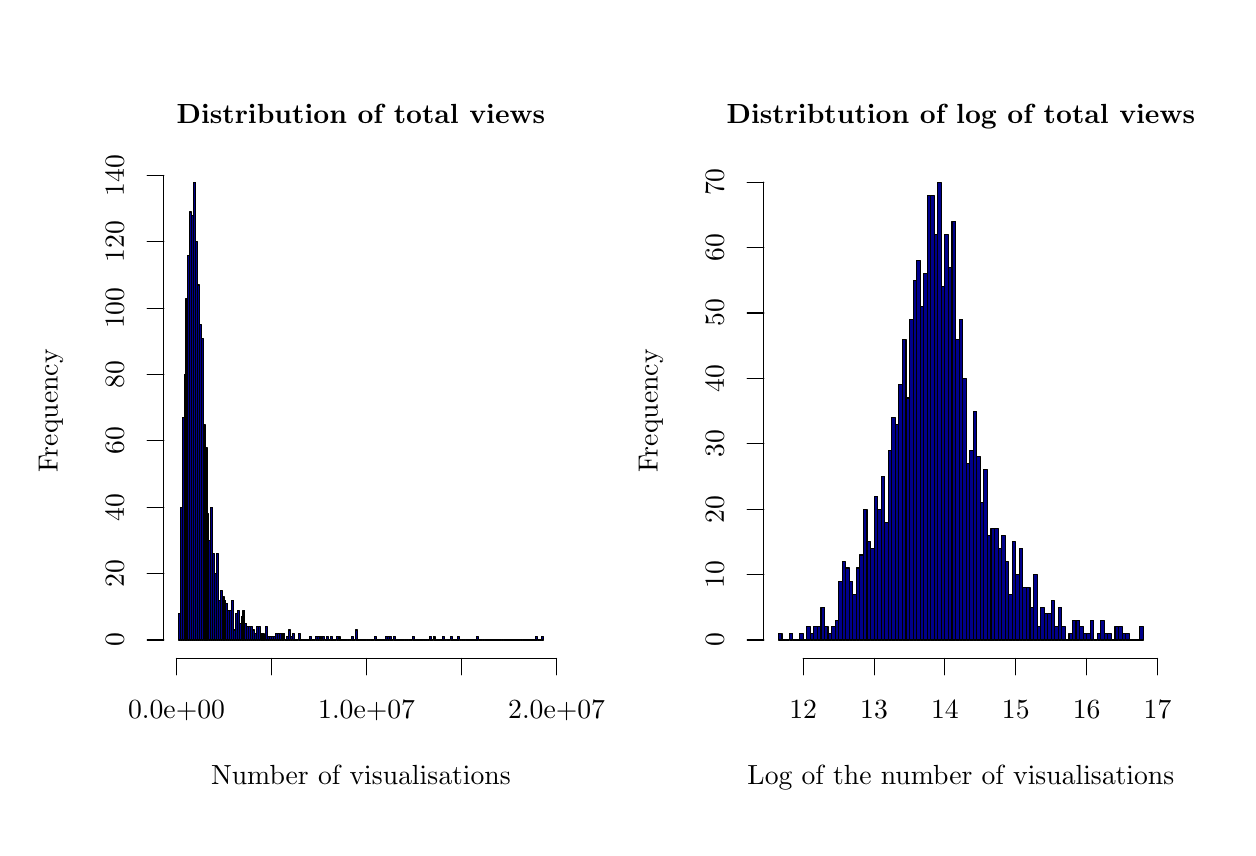
\begin{tikzpicture}[x=1pt,y=1pt]
\definecolor{fillColor}{RGB}{255,255,255}
\path[use as bounding box,fill=fillColor,fill opacity=0.00] (0,0) rectangle (433.62,289.08);
\begin{scope}
\path[clip] (  0.00,  0.00) rectangle (216.81,289.08);
\definecolor{drawColor}{RGB}{0,0,0}

\node[text=drawColor,anchor=base,inner sep=0pt, outer sep=0pt, scale=  1.00] at (120.41, 15.60) {Number of visualisations};

\node[text=drawColor,rotate= 90.00,anchor=base,inner sep=0pt, outer sep=0pt, scale=  1.00] at ( 10.80,150.54) {Frequency};
\end{scope}
\begin{scope}
\path[clip] (  0.00,  0.00) rectangle (433.62,289.08);
\definecolor{drawColor}{RGB}{0,0,0}

\path[draw=drawColor,line width= 0.4pt,line join=round,line cap=round] ( 53.79, 61.20) -- (191.14, 61.20);

\path[draw=drawColor,line width= 0.4pt,line join=round,line cap=round] ( 53.79, 61.20) -- ( 53.79, 55.20);

\path[draw=drawColor,line width= 0.4pt,line join=round,line cap=round] ( 88.13, 61.20) -- ( 88.13, 55.20);

\path[draw=drawColor,line width= 0.4pt,line join=round,line cap=round] (122.47, 61.20) -- (122.47, 55.20);

\path[draw=drawColor,line width= 0.4pt,line join=round,line cap=round] (156.80, 61.20) -- (156.80, 55.20);

\path[draw=drawColor,line width= 0.4pt,line join=round,line cap=round] (191.14, 61.20) -- (191.14, 55.20);

\node[text=drawColor,anchor=base,inner sep=0pt, outer sep=0pt, scale=  1.00] at ( 53.79, 39.60) {0.0e+00};

\node[text=drawColor,anchor=base,inner sep=0pt, outer sep=0pt, scale=  1.00] at (122.47, 39.60) {1.0e+07};

\node[text=drawColor,anchor=base,inner sep=0pt, outer sep=0pt, scale=  1.00] at (191.14, 39.60) {2.0e+07};

\path[draw=drawColor,line width= 0.4pt,line join=round,line cap=round] ( 49.20, 67.82) -- ( 49.20,235.66);

\path[draw=drawColor,line width= 0.4pt,line join=round,line cap=round] ( 49.20, 67.82) -- ( 43.20, 67.82);

\path[draw=drawColor,line width= 0.4pt,line join=round,line cap=round] ( 49.20, 91.80) -- ( 43.20, 91.80);

\path[draw=drawColor,line width= 0.4pt,line join=round,line cap=round] ( 49.20,115.77) -- ( 43.20,115.77);

\path[draw=drawColor,line width= 0.4pt,line join=round,line cap=round] ( 49.20,139.75) -- ( 43.20,139.75);

\path[draw=drawColor,line width= 0.4pt,line join=round,line cap=round] ( 49.20,163.73) -- ( 43.20,163.73);

\path[draw=drawColor,line width= 0.4pt,line join=round,line cap=round] ( 49.20,187.71) -- ( 43.20,187.71);

\path[draw=drawColor,line width= 0.4pt,line join=round,line cap=round] ( 49.20,211.68) -- ( 43.20,211.68);

\path[draw=drawColor,line width= 0.4pt,line join=round,line cap=round] ( 49.20,235.66) -- ( 43.20,235.66);

\node[text=drawColor,rotate= 90.00,anchor=base,inner sep=0pt, outer sep=0pt, scale=  1.00] at ( 34.80, 67.82) {0};

\node[text=drawColor,rotate= 90.00,anchor=base,inner sep=0pt, outer sep=0pt, scale=  1.00] at ( 34.80, 91.80) {20};

\node[text=drawColor,rotate= 90.00,anchor=base,inner sep=0pt, outer sep=0pt, scale=  1.00] at ( 34.80,115.77) {40};

\node[text=drawColor,rotate= 90.00,anchor=base,inner sep=0pt, outer sep=0pt, scale=  1.00] at ( 34.80,139.75) {60};

\node[text=drawColor,rotate= 90.00,anchor=base,inner sep=0pt, outer sep=0pt, scale=  1.00] at ( 34.80,163.73) {80};

\node[text=drawColor,rotate= 90.00,anchor=base,inner sep=0pt, outer sep=0pt, scale=  1.00] at ( 34.80,187.71) {100};

\node[text=drawColor,rotate= 90.00,anchor=base,inner sep=0pt, outer sep=0pt, scale=  1.00] at ( 34.80,211.68) {120};

\node[text=drawColor,rotate= 90.00,anchor=base,inner sep=0pt, outer sep=0pt, scale=  1.00] at ( 34.80,235.66) {140};
\end{scope}
\begin{scope}
\path[clip] ( 49.20, 61.20) rectangle (191.61,239.88);
\definecolor{drawColor}{RGB}{0,0,0}
\definecolor{fillColor}{RGB}{0,0,139}

\path[draw=drawColor,line width= 0.4pt,line join=round,line cap=round,fill=fillColor] ( 54.47, 67.82) rectangle ( 55.16, 77.41);

\path[draw=drawColor,line width= 0.4pt,line join=round,line cap=round,fill=fillColor] ( 55.16, 67.82) rectangle ( 55.85,115.77);

\path[draw=drawColor,line width= 0.4pt,line join=round,line cap=round,fill=fillColor] ( 55.85, 67.82) rectangle ( 56.53,148.14);

\path[draw=drawColor,line width= 0.4pt,line join=round,line cap=round,fill=fillColor] ( 56.53, 67.82) rectangle ( 57.22,163.73);

\path[draw=drawColor,line width= 0.4pt,line join=round,line cap=round,fill=fillColor] ( 57.22, 67.82) rectangle ( 57.91,191.30);

\path[draw=drawColor,line width= 0.4pt,line join=round,line cap=round,fill=fillColor] ( 57.91, 67.82) rectangle ( 58.60,206.89);

\path[draw=drawColor,line width= 0.4pt,line join=round,line cap=round,fill=fillColor] ( 58.60, 67.82) rectangle ( 59.28,222.47);

\path[draw=drawColor,line width= 0.4pt,line join=round,line cap=round,fill=fillColor] ( 59.28, 67.82) rectangle ( 59.97,221.27);

\path[draw=drawColor,line width= 0.4pt,line join=round,line cap=round,fill=fillColor] ( 59.97, 67.82) rectangle ( 60.66,233.26);

\path[draw=drawColor,line width= 0.4pt,line join=round,line cap=round,fill=fillColor] ( 60.66, 67.82) rectangle ( 61.34,211.68);

\path[draw=drawColor,line width= 0.4pt,line join=round,line cap=round,fill=fillColor] ( 61.34, 67.82) rectangle ( 62.03,196.10);

\path[draw=drawColor,line width= 0.4pt,line join=round,line cap=round,fill=fillColor] ( 62.03, 67.82) rectangle ( 62.72,181.71);

\path[draw=drawColor,line width= 0.4pt,line join=round,line cap=round,fill=fillColor] ( 62.72, 67.82) rectangle ( 63.40,176.92);

\path[draw=drawColor,line width= 0.4pt,line join=round,line cap=round,fill=fillColor] ( 63.40, 67.82) rectangle ( 64.09,145.74);

\path[draw=drawColor,line width= 0.4pt,line join=round,line cap=round,fill=fillColor] ( 64.09, 67.82) rectangle ( 64.78,137.35);

\path[draw=drawColor,line width= 0.4pt,line join=round,line cap=round,fill=fillColor] ( 64.78, 67.82) rectangle ( 65.46,113.37);

\path[draw=drawColor,line width= 0.4pt,line join=round,line cap=round,fill=fillColor] ( 65.46, 67.82) rectangle ( 66.15,103.78);

\path[draw=drawColor,line width= 0.4pt,line join=round,line cap=round,fill=fillColor] ( 66.15, 67.82) rectangle ( 66.84,115.77);

\path[draw=drawColor,line width= 0.4pt,line join=round,line cap=round,fill=fillColor] ( 66.84, 67.82) rectangle ( 67.52, 98.99);

\path[draw=drawColor,line width= 0.4pt,line join=round,line cap=round,fill=fillColor] ( 67.52, 67.82) rectangle ( 68.21, 91.80);

\path[draw=drawColor,line width= 0.4pt,line join=round,line cap=round,fill=fillColor] ( 68.21, 67.82) rectangle ( 68.90, 98.99);

\path[draw=drawColor,line width= 0.4pt,line join=round,line cap=round,fill=fillColor] ( 68.90, 67.82) rectangle ( 69.58, 82.20);

\path[draw=drawColor,line width= 0.4pt,line join=round,line cap=round,fill=fillColor] ( 69.58, 67.82) rectangle ( 70.27, 85.80);

\path[draw=drawColor,line width= 0.4pt,line join=round,line cap=round,fill=fillColor] ( 70.27, 67.82) rectangle ( 70.96, 83.40);

\path[draw=drawColor,line width= 0.4pt,line join=round,line cap=round,fill=fillColor] ( 70.96, 67.82) rectangle ( 71.64, 82.20);

\path[draw=drawColor,line width= 0.4pt,line join=round,line cap=round,fill=fillColor] ( 71.64, 67.82) rectangle ( 72.33, 81.01);

\path[draw=drawColor,line width= 0.4pt,line join=round,line cap=round,fill=fillColor] ( 72.33, 67.82) rectangle ( 73.02, 78.61);

\path[draw=drawColor,line width= 0.4pt,line join=round,line cap=round,fill=fillColor] ( 73.02, 67.82) rectangle ( 73.70, 78.61);

\path[draw=drawColor,line width= 0.4pt,line join=round,line cap=round,fill=fillColor] ( 73.70, 67.82) rectangle ( 74.39, 82.20);

\path[draw=drawColor,line width= 0.4pt,line join=round,line cap=round,fill=fillColor] ( 74.39, 67.82) rectangle ( 75.08, 71.41);

\path[draw=drawColor,line width= 0.4pt,line join=round,line cap=round,fill=fillColor] ( 75.08, 67.82) rectangle ( 75.76, 77.41);

\path[draw=drawColor,line width= 0.4pt,line join=round,line cap=round,fill=fillColor] ( 75.76, 67.82) rectangle ( 76.45, 78.61);

\path[draw=drawColor,line width= 0.4pt,line join=round,line cap=round,fill=fillColor] ( 76.45, 67.82) rectangle ( 77.14, 73.81);

\path[draw=drawColor,line width= 0.4pt,line join=round,line cap=round,fill=fillColor] ( 77.14, 67.82) rectangle ( 77.82, 76.21);

\path[draw=drawColor,line width= 0.4pt,line join=round,line cap=round,fill=fillColor] ( 77.82, 67.82) rectangle ( 78.51, 78.61);

\path[draw=drawColor,line width= 0.4pt,line join=round,line cap=round,fill=fillColor] ( 78.51, 67.82) rectangle ( 79.20, 73.81);

\path[draw=drawColor,line width= 0.4pt,line join=round,line cap=round,fill=fillColor] ( 79.20, 67.82) rectangle ( 79.89, 72.61);

\path[draw=drawColor,line width= 0.4pt,line join=round,line cap=round,fill=fillColor] ( 79.89, 67.82) rectangle ( 80.57, 72.61);

\path[draw=drawColor,line width= 0.4pt,line join=round,line cap=round,fill=fillColor] ( 80.57, 67.82) rectangle ( 81.26, 72.61);

\path[draw=drawColor,line width= 0.4pt,line join=round,line cap=round,fill=fillColor] ( 81.26, 67.82) rectangle ( 81.95, 71.41);

\path[draw=drawColor,line width= 0.4pt,line join=round,line cap=round,fill=fillColor] ( 81.95, 67.82) rectangle ( 82.63, 70.22);

\path[draw=drawColor,line width= 0.4pt,line join=round,line cap=round,fill=fillColor] ( 82.63, 67.82) rectangle ( 83.32, 72.61);

\path[draw=drawColor,line width= 0.4pt,line join=round,line cap=round,fill=fillColor] ( 83.32, 67.82) rectangle ( 84.01, 72.61);

\path[draw=drawColor,line width= 0.4pt,line join=round,line cap=round,fill=fillColor] ( 84.01, 67.82) rectangle ( 84.69, 70.22);

\path[draw=drawColor,line width= 0.4pt,line join=round,line cap=round,fill=fillColor] ( 84.69, 67.82) rectangle ( 85.38, 70.22);

\path[draw=drawColor,line width= 0.4pt,line join=round,line cap=round,fill=fillColor] ( 85.38, 67.82) rectangle ( 86.07, 69.02);

\path[draw=drawColor,line width= 0.4pt,line join=round,line cap=round,fill=fillColor] ( 86.07, 67.82) rectangle ( 86.75, 72.61);

\path[draw=drawColor,line width= 0.4pt,line join=round,line cap=round,fill=fillColor] ( 86.75, 67.82) rectangle ( 87.44, 69.02);

\path[draw=drawColor,line width= 0.4pt,line join=round,line cap=round,fill=fillColor] ( 87.44, 67.82) rectangle ( 88.13, 69.02);

\path[draw=drawColor,line width= 0.4pt,line join=round,line cap=round,fill=fillColor] ( 88.13, 67.82) rectangle ( 88.81, 69.02);

\path[draw=drawColor,line width= 0.4pt,line join=round,line cap=round,fill=fillColor] ( 88.81, 67.82) rectangle ( 89.50, 69.02);

\path[draw=drawColor,line width= 0.4pt,line join=round,line cap=round,fill=fillColor] ( 89.50, 67.82) rectangle ( 90.19, 70.22);

\path[draw=drawColor,line width= 0.4pt,line join=round,line cap=round,fill=fillColor] ( 90.19, 67.82) rectangle ( 90.87, 70.22);

\path[draw=drawColor,line width= 0.4pt,line join=round,line cap=round,fill=fillColor] ( 90.87, 67.82) rectangle ( 91.56, 70.22);

\path[draw=drawColor,line width= 0.4pt,line join=round,line cap=round,fill=fillColor] ( 91.56, 67.82) rectangle ( 92.25, 70.22);

\path[draw=drawColor,line width= 0.4pt,line join=round,line cap=round,fill=fillColor] ( 92.25, 67.82) rectangle ( 92.93, 70.22);

\path[draw=drawColor,line width= 0.4pt,line join=round,line cap=round,fill=fillColor] ( 92.93, 67.82) rectangle ( 93.62, 67.82);

\path[draw=drawColor,line width= 0.4pt,line join=round,line cap=round,fill=fillColor] ( 93.62, 67.82) rectangle ( 94.31, 69.02);

\path[draw=drawColor,line width= 0.4pt,line join=round,line cap=round,fill=fillColor] ( 94.31, 67.82) rectangle ( 94.99, 71.41);

\path[draw=drawColor,line width= 0.4pt,line join=round,line cap=round,fill=fillColor] ( 94.99, 67.82) rectangle ( 95.68, 69.02);

\path[draw=drawColor,line width= 0.4pt,line join=round,line cap=round,fill=fillColor] ( 95.68, 67.82) rectangle ( 96.37, 70.22);

\path[draw=drawColor,line width= 0.4pt,line join=round,line cap=round,fill=fillColor] ( 96.37, 67.82) rectangle ( 97.05, 67.82);

\path[draw=drawColor,line width= 0.4pt,line join=round,line cap=round,fill=fillColor] ( 97.05, 67.82) rectangle ( 97.74, 67.82);

\path[draw=drawColor,line width= 0.4pt,line join=round,line cap=round,fill=fillColor] ( 97.74, 67.82) rectangle ( 98.43, 70.22);

\path[draw=drawColor,line width= 0.4pt,line join=round,line cap=round,fill=fillColor] ( 98.43, 67.82) rectangle ( 99.11, 67.82);

\path[draw=drawColor,line width= 0.4pt,line join=round,line cap=round,fill=fillColor] ( 99.11, 67.82) rectangle ( 99.80, 67.82);

\path[draw=drawColor,line width= 0.4pt,line join=round,line cap=round,fill=fillColor] ( 99.80, 67.82) rectangle (100.49, 67.82);

\path[draw=drawColor,line width= 0.4pt,line join=round,line cap=round,fill=fillColor] (100.49, 67.82) rectangle (101.18, 67.82);

\path[draw=drawColor,line width= 0.4pt,line join=round,line cap=round,fill=fillColor] (101.18, 67.82) rectangle (101.86, 67.82);

\path[draw=drawColor,line width= 0.4pt,line join=round,line cap=round,fill=fillColor] (101.86, 67.82) rectangle (102.55, 69.02);

\path[draw=drawColor,line width= 0.4pt,line join=round,line cap=round,fill=fillColor] (102.55, 67.82) rectangle (103.24, 67.82);

\path[draw=drawColor,line width= 0.4pt,line join=round,line cap=round,fill=fillColor] (103.24, 67.82) rectangle (103.92, 67.82);

\path[draw=drawColor,line width= 0.4pt,line join=round,line cap=round,fill=fillColor] (103.92, 67.82) rectangle (104.61, 69.02);

\path[draw=drawColor,line width= 0.4pt,line join=round,line cap=round,fill=fillColor] (104.61, 67.82) rectangle (105.30, 69.02);

\path[draw=drawColor,line width= 0.4pt,line join=round,line cap=round,fill=fillColor] (105.30, 67.82) rectangle (105.98, 69.02);

\path[draw=drawColor,line width= 0.4pt,line join=round,line cap=round,fill=fillColor] (105.98, 67.82) rectangle (106.67, 69.02);

\path[draw=drawColor,line width= 0.4pt,line join=round,line cap=round,fill=fillColor] (106.67, 67.82) rectangle (107.36, 69.02);

\path[draw=drawColor,line width= 0.4pt,line join=round,line cap=round,fill=fillColor] (107.36, 67.82) rectangle (108.04, 67.82);

\path[draw=drawColor,line width= 0.4pt,line join=round,line cap=round,fill=fillColor] (108.04, 67.82) rectangle (108.73, 69.02);

\path[draw=drawColor,line width= 0.4pt,line join=round,line cap=round,fill=fillColor] (108.73, 67.82) rectangle (109.42, 67.82);

\path[draw=drawColor,line width= 0.4pt,line join=round,line cap=round,fill=fillColor] (109.42, 67.82) rectangle (110.10, 69.02);

\path[draw=drawColor,line width= 0.4pt,line join=round,line cap=round,fill=fillColor] (110.10, 67.82) rectangle (110.79, 67.82);

\path[draw=drawColor,line width= 0.4pt,line join=round,line cap=round,fill=fillColor] (110.79, 67.82) rectangle (111.48, 67.82);

\path[draw=drawColor,line width= 0.4pt,line join=round,line cap=round,fill=fillColor] (111.48, 67.82) rectangle (112.16, 69.02);

\path[draw=drawColor,line width= 0.4pt,line join=round,line cap=round,fill=fillColor] (112.16, 67.82) rectangle (112.85, 69.02);

\path[draw=drawColor,line width= 0.4pt,line join=round,line cap=round,fill=fillColor] (112.85, 67.82) rectangle (113.54, 67.82);

\path[draw=drawColor,line width= 0.4pt,line join=round,line cap=round,fill=fillColor] (113.54, 67.82) rectangle (114.22, 67.82);

\path[draw=drawColor,line width= 0.4pt,line join=round,line cap=round,fill=fillColor] (114.22, 67.82) rectangle (114.91, 67.82);

\path[draw=drawColor,line width= 0.4pt,line join=round,line cap=round,fill=fillColor] (114.91, 67.82) rectangle (115.60, 67.82);

\path[draw=drawColor,line width= 0.4pt,line join=round,line cap=round,fill=fillColor] (115.60, 67.82) rectangle (116.28, 67.82);

\path[draw=drawColor,line width= 0.4pt,line join=round,line cap=round,fill=fillColor] (116.28, 67.82) rectangle (116.97, 67.82);

\path[draw=drawColor,line width= 0.4pt,line join=round,line cap=round,fill=fillColor] (116.97, 67.82) rectangle (117.66, 69.02);

\path[draw=drawColor,line width= 0.4pt,line join=round,line cap=round,fill=fillColor] (117.66, 67.82) rectangle (118.34, 67.82);

\path[draw=drawColor,line width= 0.4pt,line join=round,line cap=round,fill=fillColor] (118.34, 67.82) rectangle (119.03, 71.41);

\path[draw=drawColor,line width= 0.4pt,line join=round,line cap=round,fill=fillColor] (119.03, 67.82) rectangle (119.72, 67.82);

\path[draw=drawColor,line width= 0.4pt,line join=round,line cap=round,fill=fillColor] (119.72, 67.82) rectangle (120.41, 67.82);

\path[draw=drawColor,line width= 0.4pt,line join=round,line cap=round,fill=fillColor] (120.41, 67.82) rectangle (121.09, 67.82);

\path[draw=drawColor,line width= 0.4pt,line join=round,line cap=round,fill=fillColor] (121.09, 67.82) rectangle (121.78, 67.82);

\path[draw=drawColor,line width= 0.4pt,line join=round,line cap=round,fill=fillColor] (121.78, 67.82) rectangle (122.47, 67.82);

\path[draw=drawColor,line width= 0.4pt,line join=round,line cap=round,fill=fillColor] (122.47, 67.82) rectangle (123.15, 67.82);

\path[draw=drawColor,line width= 0.4pt,line join=round,line cap=round,fill=fillColor] (123.15, 67.82) rectangle (123.84, 67.82);

\path[draw=drawColor,line width= 0.4pt,line join=round,line cap=round,fill=fillColor] (123.84, 67.82) rectangle (124.53, 67.82);

\path[draw=drawColor,line width= 0.4pt,line join=round,line cap=round,fill=fillColor] (124.53, 67.82) rectangle (125.21, 67.82);

\path[draw=drawColor,line width= 0.4pt,line join=round,line cap=round,fill=fillColor] (125.21, 67.82) rectangle (125.90, 69.02);

\path[draw=drawColor,line width= 0.4pt,line join=round,line cap=round,fill=fillColor] (125.90, 67.82) rectangle (126.59, 67.82);

\path[draw=drawColor,line width= 0.4pt,line join=round,line cap=round,fill=fillColor] (126.59, 67.82) rectangle (127.27, 67.82);

\path[draw=drawColor,line width= 0.4pt,line join=round,line cap=round,fill=fillColor] (127.27, 67.82) rectangle (127.96, 67.82);

\path[draw=drawColor,line width= 0.4pt,line join=round,line cap=round,fill=fillColor] (127.96, 67.82) rectangle (128.65, 67.82);

\path[draw=drawColor,line width= 0.4pt,line join=round,line cap=round,fill=fillColor] (128.65, 67.82) rectangle (129.33, 67.82);

\path[draw=drawColor,line width= 0.4pt,line join=round,line cap=round,fill=fillColor] (129.33, 67.82) rectangle (130.02, 69.02);

\path[draw=drawColor,line width= 0.4pt,line join=round,line cap=round,fill=fillColor] (130.02, 67.82) rectangle (130.71, 69.02);

\path[draw=drawColor,line width= 0.4pt,line join=round,line cap=round,fill=fillColor] (130.71, 67.82) rectangle (131.39, 69.02);

\path[draw=drawColor,line width= 0.4pt,line join=round,line cap=round,fill=fillColor] (131.39, 67.82) rectangle (132.08, 67.82);

\path[draw=drawColor,line width= 0.4pt,line join=round,line cap=round,fill=fillColor] (132.08, 67.82) rectangle (132.77, 69.02);

\path[draw=drawColor,line width= 0.4pt,line join=round,line cap=round,fill=fillColor] (132.77, 67.82) rectangle (133.45, 67.82);

\path[draw=drawColor,line width= 0.4pt,line join=round,line cap=round,fill=fillColor] (133.45, 67.82) rectangle (134.14, 67.82);

\path[draw=drawColor,line width= 0.4pt,line join=round,line cap=round,fill=fillColor] (134.14, 67.82) rectangle (134.83, 67.82);

\path[draw=drawColor,line width= 0.4pt,line join=round,line cap=round,fill=fillColor] (134.83, 67.82) rectangle (135.51, 67.82);

\path[draw=drawColor,line width= 0.4pt,line join=round,line cap=round,fill=fillColor] (135.51, 67.82) rectangle (136.20, 67.82);

\path[draw=drawColor,line width= 0.4pt,line join=round,line cap=round,fill=fillColor] (136.20, 67.82) rectangle (136.89, 67.82);

\path[draw=drawColor,line width= 0.4pt,line join=round,line cap=round,fill=fillColor] (136.89, 67.82) rectangle (137.57, 67.82);

\path[draw=drawColor,line width= 0.4pt,line join=round,line cap=round,fill=fillColor] (137.57, 67.82) rectangle (138.26, 67.82);

\path[draw=drawColor,line width= 0.4pt,line join=round,line cap=round,fill=fillColor] (138.26, 67.82) rectangle (138.95, 67.82);

\path[draw=drawColor,line width= 0.4pt,line join=round,line cap=round,fill=fillColor] (138.95, 67.82) rectangle (139.63, 69.02);

\path[draw=drawColor,line width= 0.4pt,line join=round,line cap=round,fill=fillColor] (139.63, 67.82) rectangle (140.32, 67.82);

\path[draw=drawColor,line width= 0.4pt,line join=round,line cap=round,fill=fillColor] (140.32, 67.82) rectangle (141.01, 67.82);

\path[draw=drawColor,line width= 0.4pt,line join=round,line cap=round,fill=fillColor] (141.01, 67.82) rectangle (141.70, 67.82);

\path[draw=drawColor,line width= 0.4pt,line join=round,line cap=round,fill=fillColor] (141.70, 67.82) rectangle (142.38, 67.82);

\path[draw=drawColor,line width= 0.4pt,line join=round,line cap=round,fill=fillColor] (142.38, 67.82) rectangle (143.07, 67.82);

\path[draw=drawColor,line width= 0.4pt,line join=round,line cap=round,fill=fillColor] (143.07, 67.82) rectangle (143.76, 67.82);

\path[draw=drawColor,line width= 0.4pt,line join=round,line cap=round,fill=fillColor] (143.76, 67.82) rectangle (144.44, 67.82);

\path[draw=drawColor,line width= 0.4pt,line join=round,line cap=round,fill=fillColor] (144.44, 67.82) rectangle (145.13, 67.82);

\path[draw=drawColor,line width= 0.4pt,line join=round,line cap=round,fill=fillColor] (145.13, 67.82) rectangle (145.82, 69.02);

\path[draw=drawColor,line width= 0.4pt,line join=round,line cap=round,fill=fillColor] (145.82, 67.82) rectangle (146.50, 67.82);

\path[draw=drawColor,line width= 0.4pt,line join=round,line cap=round,fill=fillColor] (146.50, 67.82) rectangle (147.19, 69.02);

\path[draw=drawColor,line width= 0.4pt,line join=round,line cap=round,fill=fillColor] (147.19, 67.82) rectangle (147.88, 67.82);

\path[draw=drawColor,line width= 0.4pt,line join=round,line cap=round,fill=fillColor] (147.88, 67.82) rectangle (148.56, 67.82);

\path[draw=drawColor,line width= 0.4pt,line join=round,line cap=round,fill=fillColor] (148.56, 67.82) rectangle (149.25, 67.82);

\path[draw=drawColor,line width= 0.4pt,line join=round,line cap=round,fill=fillColor] (149.25, 67.82) rectangle (149.94, 67.82);

\path[draw=drawColor,line width= 0.4pt,line join=round,line cap=round,fill=fillColor] (149.94, 67.82) rectangle (150.62, 69.02);

\path[draw=drawColor,line width= 0.4pt,line join=round,line cap=round,fill=fillColor] (150.62, 67.82) rectangle (151.31, 67.82);

\path[draw=drawColor,line width= 0.4pt,line join=round,line cap=round,fill=fillColor] (151.31, 67.82) rectangle (152.00, 67.82);

\path[draw=drawColor,line width= 0.4pt,line join=round,line cap=round,fill=fillColor] (152.00, 67.82) rectangle (152.68, 67.82);

\path[draw=drawColor,line width= 0.4pt,line join=round,line cap=round,fill=fillColor] (152.68, 67.82) rectangle (153.37, 69.02);

\path[draw=drawColor,line width= 0.4pt,line join=round,line cap=round,fill=fillColor] (153.37, 67.82) rectangle (154.06, 67.82);

\path[draw=drawColor,line width= 0.4pt,line join=round,line cap=round,fill=fillColor] (154.06, 67.82) rectangle (154.74, 67.82);

\path[draw=drawColor,line width= 0.4pt,line join=round,line cap=round,fill=fillColor] (154.74, 67.82) rectangle (155.43, 67.82);

\path[draw=drawColor,line width= 0.4pt,line join=round,line cap=round,fill=fillColor] (155.43, 67.82) rectangle (156.12, 69.02);

\path[draw=drawColor,line width= 0.4pt,line join=round,line cap=round,fill=fillColor] (156.12, 67.82) rectangle (156.80, 67.82);

\path[draw=drawColor,line width= 0.4pt,line join=round,line cap=round,fill=fillColor] (156.80, 67.82) rectangle (157.49, 67.82);

\path[draw=drawColor,line width= 0.4pt,line join=round,line cap=round,fill=fillColor] (157.49, 67.82) rectangle (158.18, 67.82);

\path[draw=drawColor,line width= 0.4pt,line join=round,line cap=round,fill=fillColor] (158.18, 67.82) rectangle (158.86, 67.82);

\path[draw=drawColor,line width= 0.4pt,line join=round,line cap=round,fill=fillColor] (158.86, 67.82) rectangle (159.55, 67.82);

\path[draw=drawColor,line width= 0.4pt,line join=round,line cap=round,fill=fillColor] (159.55, 67.82) rectangle (160.24, 67.82);

\path[draw=drawColor,line width= 0.4pt,line join=round,line cap=round,fill=fillColor] (160.24, 67.82) rectangle (160.92, 67.82);

\path[draw=drawColor,line width= 0.4pt,line join=round,line cap=round,fill=fillColor] (160.92, 67.82) rectangle (161.61, 67.82);

\path[draw=drawColor,line width= 0.4pt,line join=round,line cap=round,fill=fillColor] (161.61, 67.82) rectangle (162.30, 67.82);

\path[draw=drawColor,line width= 0.4pt,line join=round,line cap=round,fill=fillColor] (162.30, 67.82) rectangle (162.99, 69.02);

\path[draw=drawColor,line width= 0.4pt,line join=round,line cap=round,fill=fillColor] (162.99, 67.82) rectangle (163.67, 67.82);

\path[draw=drawColor,line width= 0.4pt,line join=round,line cap=round,fill=fillColor] (163.67, 67.82) rectangle (164.36, 67.82);

\path[draw=drawColor,line width= 0.4pt,line join=round,line cap=round,fill=fillColor] (164.36, 67.82) rectangle (165.05, 67.82);

\path[draw=drawColor,line width= 0.4pt,line join=round,line cap=round,fill=fillColor] (165.05, 67.82) rectangle (165.73, 67.82);

\path[draw=drawColor,line width= 0.4pt,line join=round,line cap=round,fill=fillColor] (165.73, 67.82) rectangle (166.42, 67.82);

\path[draw=drawColor,line width= 0.4pt,line join=round,line cap=round,fill=fillColor] (166.42, 67.82) rectangle (167.11, 67.82);

\path[draw=drawColor,line width= 0.4pt,line join=round,line cap=round,fill=fillColor] (167.11, 67.82) rectangle (167.79, 67.82);

\path[draw=drawColor,line width= 0.4pt,line join=round,line cap=round,fill=fillColor] (167.79, 67.82) rectangle (168.48, 67.82);

\path[draw=drawColor,line width= 0.4pt,line join=round,line cap=round,fill=fillColor] (168.48, 67.82) rectangle (169.17, 67.82);

\path[draw=drawColor,line width= 0.4pt,line join=round,line cap=round,fill=fillColor] (169.17, 67.82) rectangle (169.85, 67.82);

\path[draw=drawColor,line width= 0.4pt,line join=round,line cap=round,fill=fillColor] (169.85, 67.82) rectangle (170.54, 67.82);

\path[draw=drawColor,line width= 0.4pt,line join=round,line cap=round,fill=fillColor] (170.54, 67.82) rectangle (171.23, 67.82);

\path[draw=drawColor,line width= 0.4pt,line join=round,line cap=round,fill=fillColor] (171.23, 67.82) rectangle (171.91, 67.82);

\path[draw=drawColor,line width= 0.4pt,line join=round,line cap=round,fill=fillColor] (171.91, 67.82) rectangle (172.60, 67.82);

\path[draw=drawColor,line width= 0.4pt,line join=round,line cap=round,fill=fillColor] (172.60, 67.82) rectangle (173.29, 67.82);

\path[draw=drawColor,line width= 0.4pt,line join=round,line cap=round,fill=fillColor] (173.29, 67.82) rectangle (173.97, 67.82);

\path[draw=drawColor,line width= 0.4pt,line join=round,line cap=round,fill=fillColor] (173.97, 67.82) rectangle (174.66, 67.82);

\path[draw=drawColor,line width= 0.4pt,line join=round,line cap=round,fill=fillColor] (174.66, 67.82) rectangle (175.35, 67.82);

\path[draw=drawColor,line width= 0.4pt,line join=round,line cap=round,fill=fillColor] (175.35, 67.82) rectangle (176.03, 67.82);

\path[draw=drawColor,line width= 0.4pt,line join=round,line cap=round,fill=fillColor] (176.03, 67.82) rectangle (176.72, 67.82);

\path[draw=drawColor,line width= 0.4pt,line join=round,line cap=round,fill=fillColor] (176.72, 67.82) rectangle (177.41, 67.82);

\path[draw=drawColor,line width= 0.4pt,line join=round,line cap=round,fill=fillColor] (177.41, 67.82) rectangle (178.09, 67.82);

\path[draw=drawColor,line width= 0.4pt,line join=round,line cap=round,fill=fillColor] (178.09, 67.82) rectangle (178.78, 67.82);

\path[draw=drawColor,line width= 0.4pt,line join=round,line cap=round,fill=fillColor] (178.78, 67.82) rectangle (179.47, 67.82);

\path[draw=drawColor,line width= 0.4pt,line join=round,line cap=round,fill=fillColor] (179.47, 67.82) rectangle (180.15, 67.82);

\path[draw=drawColor,line width= 0.4pt,line join=round,line cap=round,fill=fillColor] (180.15, 67.82) rectangle (180.84, 67.82);

\path[draw=drawColor,line width= 0.4pt,line join=round,line cap=round,fill=fillColor] (180.84, 67.82) rectangle (181.53, 67.82);

\path[draw=drawColor,line width= 0.4pt,line join=round,line cap=round,fill=fillColor] (181.53, 67.82) rectangle (182.21, 67.82);

\path[draw=drawColor,line width= 0.4pt,line join=round,line cap=round,fill=fillColor] (182.21, 67.82) rectangle (182.90, 67.82);

\path[draw=drawColor,line width= 0.4pt,line join=round,line cap=round,fill=fillColor] (182.90, 67.82) rectangle (183.59, 67.82);

\path[draw=drawColor,line width= 0.4pt,line join=round,line cap=round,fill=fillColor] (183.59, 67.82) rectangle (184.28, 69.02);

\path[draw=drawColor,line width= 0.4pt,line join=round,line cap=round,fill=fillColor] (184.28, 67.82) rectangle (184.96, 67.82);

\path[draw=drawColor,line width= 0.4pt,line join=round,line cap=round,fill=fillColor] (184.96, 67.82) rectangle (185.65, 67.82);

\path[draw=drawColor,line width= 0.4pt,line join=round,line cap=round,fill=fillColor] (185.65, 67.82) rectangle (186.34, 69.02);
\end{scope}
\begin{scope}
\path[clip] (  0.00,  0.00) rectangle (433.62,289.08);
\definecolor{drawColor}{RGB}{0,0,0}

\node[text=drawColor,anchor=base,inner sep=0pt, outer sep=0pt, scale=  1.00] at (120.41,254.28) {\textbf{Distribution of total views}};
\end{scope}
\begin{scope}
\path[clip] (216.81,  0.00) rectangle (433.62,289.08);
\definecolor{drawColor}{RGB}{0,0,0}

\node[text=drawColor,anchor=base,inner sep=0pt, outer sep=0pt, scale=  1.00] at (337.21, 15.60) {Log of the number of visualisations};

\node[text=drawColor,rotate= 90.00,anchor=base,inner sep=0pt, outer sep=0pt, scale=  1.00] at (227.61,150.54) {Frequency};
\end{scope}
\begin{scope}
\path[clip] (  0.00,  0.00) rectangle (433.62,289.08);
\definecolor{drawColor}{RGB}{0,0,0}

\path[draw=drawColor,line width= 0.4pt,line join=round,line cap=round] (280.25, 61.20) -- (408.27, 61.20);

\path[draw=drawColor,line width= 0.4pt,line join=round,line cap=round] (280.25, 61.20) -- (280.25, 55.20);

\path[draw=drawColor,line width= 0.4pt,line join=round,line cap=round] (305.85, 61.20) -- (305.85, 55.20);

\path[draw=drawColor,line width= 0.4pt,line join=round,line cap=round] (331.45, 61.20) -- (331.45, 55.20);

\path[draw=drawColor,line width= 0.4pt,line join=round,line cap=round] (357.06, 61.20) -- (357.06, 55.20);

\path[draw=drawColor,line width= 0.4pt,line join=round,line cap=round] (382.66, 61.20) -- (382.66, 55.20);

\path[draw=drawColor,line width= 0.4pt,line join=round,line cap=round] (408.27, 61.20) -- (408.27, 55.20);

\node[text=drawColor,anchor=base,inner sep=0pt, outer sep=0pt, scale=  1.00] at (280.25, 39.60) {12};

\node[text=drawColor,anchor=base,inner sep=0pt, outer sep=0pt, scale=  1.00] at (305.85, 39.60) {13};

\node[text=drawColor,anchor=base,inner sep=0pt, outer sep=0pt, scale=  1.00] at (331.45, 39.60) {14};

\node[text=drawColor,anchor=base,inner sep=0pt, outer sep=0pt, scale=  1.00] at (357.06, 39.60) {15};

\node[text=drawColor,anchor=base,inner sep=0pt, outer sep=0pt, scale=  1.00] at (382.66, 39.60) {16};

\node[text=drawColor,anchor=base,inner sep=0pt, outer sep=0pt, scale=  1.00] at (408.27, 39.60) {17};

\path[draw=drawColor,line width= 0.4pt,line join=round,line cap=round] (266.01, 67.82) -- (266.01,233.26);

\path[draw=drawColor,line width= 0.4pt,line join=round,line cap=round] (266.01, 67.82) -- (260.01, 67.82);

\path[draw=drawColor,line width= 0.4pt,line join=round,line cap=round] (266.01, 91.45) -- (260.01, 91.45);

\path[draw=drawColor,line width= 0.4pt,line join=round,line cap=round] (266.01,115.09) -- (260.01,115.09);

\path[draw=drawColor,line width= 0.4pt,line join=round,line cap=round] (266.01,138.72) -- (260.01,138.72);

\path[draw=drawColor,line width= 0.4pt,line join=round,line cap=round] (266.01,162.36) -- (260.01,162.36);

\path[draw=drawColor,line width= 0.4pt,line join=round,line cap=round] (266.01,185.99) -- (260.01,185.99);

\path[draw=drawColor,line width= 0.4pt,line join=round,line cap=round] (266.01,209.63) -- (260.01,209.63);

\path[draw=drawColor,line width= 0.4pt,line join=round,line cap=round] (266.01,233.26) -- (260.01,233.26);

\node[text=drawColor,rotate= 90.00,anchor=base,inner sep=0pt, outer sep=0pt, scale=  1.00] at (251.61, 67.82) {0};

\node[text=drawColor,rotate= 90.00,anchor=base,inner sep=0pt, outer sep=0pt, scale=  1.00] at (251.61, 91.45) {10};

\node[text=drawColor,rotate= 90.00,anchor=base,inner sep=0pt, outer sep=0pt, scale=  1.00] at (251.61,115.09) {20};

\node[text=drawColor,rotate= 90.00,anchor=base,inner sep=0pt, outer sep=0pt, scale=  1.00] at (251.61,138.72) {30};

\node[text=drawColor,rotate= 90.00,anchor=base,inner sep=0pt, outer sep=0pt, scale=  1.00] at (251.61,162.36) {40};

\node[text=drawColor,rotate= 90.00,anchor=base,inner sep=0pt, outer sep=0pt, scale=  1.00] at (251.61,185.99) {50};

\node[text=drawColor,rotate= 90.00,anchor=base,inner sep=0pt, outer sep=0pt, scale=  1.00] at (251.61,209.63) {60};

\node[text=drawColor,rotate= 90.00,anchor=base,inner sep=0pt, outer sep=0pt, scale=  1.00] at (251.61,233.26) {70};
\end{scope}
\begin{scope}
\path[clip] (266.01, 61.20) rectangle (408.42,239.88);
\definecolor{drawColor}{RGB}{0,0,0}
\definecolor{fillColor}{RGB}{0,0,139}

\path[draw=drawColor,line width= 0.4pt,line join=round,line cap=round,fill=fillColor] (271.28, 67.82) rectangle (272.56, 70.18);

\path[draw=drawColor,line width= 0.4pt,line join=round,line cap=round,fill=fillColor] (272.56, 67.82) rectangle (273.84, 67.82);

\path[draw=drawColor,line width= 0.4pt,line join=round,line cap=round,fill=fillColor] (273.84, 67.82) rectangle (275.13, 67.82);

\path[draw=drawColor,line width= 0.4pt,line join=round,line cap=round,fill=fillColor] (275.13, 67.82) rectangle (276.41, 70.18);

\path[draw=drawColor,line width= 0.4pt,line join=round,line cap=round,fill=fillColor] (276.41, 67.82) rectangle (277.69, 67.82);

\path[draw=drawColor,line width= 0.4pt,line join=round,line cap=round,fill=fillColor] (277.69, 67.82) rectangle (278.97, 67.82);

\path[draw=drawColor,line width= 0.4pt,line join=round,line cap=round,fill=fillColor] (278.97, 67.82) rectangle (280.25, 70.18);

\path[draw=drawColor,line width= 0.4pt,line join=round,line cap=round,fill=fillColor] (280.25, 67.82) rectangle (281.53, 67.82);

\path[draw=drawColor,line width= 0.4pt,line join=round,line cap=round,fill=fillColor] (281.53, 67.82) rectangle (282.81, 72.54);

\path[draw=drawColor,line width= 0.4pt,line join=round,line cap=round,fill=fillColor] (282.81, 67.82) rectangle (284.09, 70.18);

\path[draw=drawColor,line width= 0.4pt,line join=round,line cap=round,fill=fillColor] (284.09, 67.82) rectangle (285.37, 72.54);

\path[draw=drawColor,line width= 0.4pt,line join=round,line cap=round,fill=fillColor] (285.37, 67.82) rectangle (286.65, 72.54);

\path[draw=drawColor,line width= 0.4pt,line join=round,line cap=round,fill=fillColor] (286.65, 67.82) rectangle (287.93, 79.64);

\path[draw=drawColor,line width= 0.4pt,line join=round,line cap=round,fill=fillColor] (287.93, 67.82) rectangle (289.21, 72.54);

\path[draw=drawColor,line width= 0.4pt,line join=round,line cap=round,fill=fillColor] (289.21, 67.82) rectangle (290.49, 70.18);

\path[draw=drawColor,line width= 0.4pt,line join=round,line cap=round,fill=fillColor] (290.49, 67.82) rectangle (291.77, 72.54);

\path[draw=drawColor,line width= 0.4pt,line join=round,line cap=round,fill=fillColor] (291.77, 67.82) rectangle (293.05, 74.91);

\path[draw=drawColor,line width= 0.4pt,line join=round,line cap=round,fill=fillColor] (293.05, 67.82) rectangle (294.33, 89.09);

\path[draw=drawColor,line width= 0.4pt,line join=round,line cap=round,fill=fillColor] (294.33, 67.82) rectangle (295.61, 96.18);

\path[draw=drawColor,line width= 0.4pt,line join=round,line cap=round,fill=fillColor] (295.61, 67.82) rectangle (296.89, 93.82);

\path[draw=drawColor,line width= 0.4pt,line join=round,line cap=round,fill=fillColor] (296.89, 67.82) rectangle (298.17, 89.09);

\path[draw=drawColor,line width= 0.4pt,line join=round,line cap=round,fill=fillColor] (298.17, 67.82) rectangle (299.45, 84.36);

\path[draw=drawColor,line width= 0.4pt,line join=round,line cap=round,fill=fillColor] (299.45, 67.82) rectangle (300.73, 93.82);

\path[draw=drawColor,line width= 0.4pt,line join=round,line cap=round,fill=fillColor] (300.73, 67.82) rectangle (302.01, 98.54);

\path[draw=drawColor,line width= 0.4pt,line join=round,line cap=round,fill=fillColor] (302.01, 67.82) rectangle (303.29,115.09);

\path[draw=drawColor,line width= 0.4pt,line join=round,line cap=round,fill=fillColor] (303.29, 67.82) rectangle (304.57,103.27);

\path[draw=drawColor,line width= 0.4pt,line join=round,line cap=round,fill=fillColor] (304.57, 67.82) rectangle (305.85,100.91);

\path[draw=drawColor,line width= 0.4pt,line join=round,line cap=round,fill=fillColor] (305.85, 67.82) rectangle (307.13,119.81);

\path[draw=drawColor,line width= 0.4pt,line join=round,line cap=round,fill=fillColor] (307.13, 67.82) rectangle (308.41,115.09);

\path[draw=drawColor,line width= 0.4pt,line join=round,line cap=round,fill=fillColor] (308.41, 67.82) rectangle (309.69,126.91);

\path[draw=drawColor,line width= 0.4pt,line join=round,line cap=round,fill=fillColor] (309.69, 67.82) rectangle (310.97,110.36);

\path[draw=drawColor,line width= 0.4pt,line join=round,line cap=round,fill=fillColor] (310.97, 67.82) rectangle (312.25,136.36);

\path[draw=drawColor,line width= 0.4pt,line join=round,line cap=round,fill=fillColor] (312.25, 67.82) rectangle (313.53,148.18);

\path[draw=drawColor,line width= 0.4pt,line join=round,line cap=round,fill=fillColor] (313.53, 67.82) rectangle (314.81,145.81);

\path[draw=drawColor,line width= 0.4pt,line join=round,line cap=round,fill=fillColor] (314.81, 67.82) rectangle (316.09,159.99);

\path[draw=drawColor,line width= 0.4pt,line join=round,line cap=round,fill=fillColor] (316.09, 67.82) rectangle (317.37,176.54);

\path[draw=drawColor,line width= 0.4pt,line join=round,line cap=round,fill=fillColor] (317.37, 67.82) rectangle (318.65,155.27);

\path[draw=drawColor,line width= 0.4pt,line join=round,line cap=round,fill=fillColor] (318.65, 67.82) rectangle (319.93,183.63);

\path[draw=drawColor,line width= 0.4pt,line join=round,line cap=round,fill=fillColor] (319.93, 67.82) rectangle (321.21,197.81);

\path[draw=drawColor,line width= 0.4pt,line join=round,line cap=round,fill=fillColor] (321.21, 67.82) rectangle (322.49,204.90);

\path[draw=drawColor,line width= 0.4pt,line join=round,line cap=round,fill=fillColor] (322.49, 67.82) rectangle (323.77,188.36);

\path[draw=drawColor,line width= 0.4pt,line join=round,line cap=round,fill=fillColor] (323.77, 67.82) rectangle (325.05,200.17);

\path[draw=drawColor,line width= 0.4pt,line join=round,line cap=round,fill=fillColor] (325.05, 67.82) rectangle (326.33,228.54);

\path[draw=drawColor,line width= 0.4pt,line join=round,line cap=round,fill=fillColor] (326.33, 67.82) rectangle (327.61,228.54);

\path[draw=drawColor,line width= 0.4pt,line join=round,line cap=round,fill=fillColor] (327.61, 67.82) rectangle (328.89,214.35);

\path[draw=drawColor,line width= 0.4pt,line join=round,line cap=round,fill=fillColor] (328.89, 67.82) rectangle (330.17,233.26);

\path[draw=drawColor,line width= 0.4pt,line join=round,line cap=round,fill=fillColor] (330.17, 67.82) rectangle (331.45,195.45);

\path[draw=drawColor,line width= 0.4pt,line join=round,line cap=round,fill=fillColor] (331.45, 67.82) rectangle (332.73,214.35);

\path[draw=drawColor,line width= 0.4pt,line join=round,line cap=round,fill=fillColor] (332.73, 67.82) rectangle (334.01,202.54);

\path[draw=drawColor,line width= 0.4pt,line join=round,line cap=round,fill=fillColor] (334.01, 67.82) rectangle (335.29,219.08);

\path[draw=drawColor,line width= 0.4pt,line join=round,line cap=round,fill=fillColor] (335.29, 67.82) rectangle (336.57,176.54);

\path[draw=drawColor,line width= 0.4pt,line join=round,line cap=round,fill=fillColor] (336.57, 67.82) rectangle (337.86,183.63);

\path[draw=drawColor,line width= 0.4pt,line join=round,line cap=round,fill=fillColor] (337.86, 67.82) rectangle (339.14,162.36);

\path[draw=drawColor,line width= 0.4pt,line join=round,line cap=round,fill=fillColor] (339.14, 67.82) rectangle (340.42,131.63);

\path[draw=drawColor,line width= 0.4pt,line join=round,line cap=round,fill=fillColor] (340.42, 67.82) rectangle (341.70,136.36);

\path[draw=drawColor,line width= 0.4pt,line join=round,line cap=round,fill=fillColor] (341.70, 67.82) rectangle (342.98,150.54);

\path[draw=drawColor,line width= 0.4pt,line join=round,line cap=round,fill=fillColor] (342.98, 67.82) rectangle (344.26,134.00);

\path[draw=drawColor,line width= 0.4pt,line join=round,line cap=round,fill=fillColor] (344.26, 67.82) rectangle (345.54,117.45);

\path[draw=drawColor,line width= 0.4pt,line join=round,line cap=round,fill=fillColor] (345.54, 67.82) rectangle (346.82,129.27);

\path[draw=drawColor,line width= 0.4pt,line join=round,line cap=round,fill=fillColor] (346.82, 67.82) rectangle (348.10,105.63);

\path[draw=drawColor,line width= 0.4pt,line join=round,line cap=round,fill=fillColor] (348.10, 67.82) rectangle (349.38,108.00);

\path[draw=drawColor,line width= 0.4pt,line join=round,line cap=round,fill=fillColor] (349.38, 67.82) rectangle (350.66,108.00);

\path[draw=drawColor,line width= 0.4pt,line join=round,line cap=round,fill=fillColor] (350.66, 67.82) rectangle (351.94,100.91);

\path[draw=drawColor,line width= 0.4pt,line join=round,line cap=round,fill=fillColor] (351.94, 67.82) rectangle (353.22,105.63);

\path[draw=drawColor,line width= 0.4pt,line join=round,line cap=round,fill=fillColor] (353.22, 67.82) rectangle (354.50, 96.18);

\path[draw=drawColor,line width= 0.4pt,line join=round,line cap=round,fill=fillColor] (354.50, 67.82) rectangle (355.78, 84.36);

\path[draw=drawColor,line width= 0.4pt,line join=round,line cap=round,fill=fillColor] (355.78, 67.82) rectangle (357.06,103.27);

\path[draw=drawColor,line width= 0.4pt,line join=round,line cap=round,fill=fillColor] (357.06, 67.82) rectangle (358.34, 91.45);

\path[draw=drawColor,line width= 0.4pt,line join=round,line cap=round,fill=fillColor] (358.34, 67.82) rectangle (359.62,100.91);

\path[draw=drawColor,line width= 0.4pt,line join=round,line cap=round,fill=fillColor] (359.62, 67.82) rectangle (360.90, 86.73);

\path[draw=drawColor,line width= 0.4pt,line join=round,line cap=round,fill=fillColor] (360.90, 67.82) rectangle (362.18, 86.73);

\path[draw=drawColor,line width= 0.4pt,line join=round,line cap=round,fill=fillColor] (362.18, 67.82) rectangle (363.46, 79.64);

\path[draw=drawColor,line width= 0.4pt,line join=round,line cap=round,fill=fillColor] (363.46, 67.82) rectangle (364.74, 91.45);

\path[draw=drawColor,line width= 0.4pt,line join=round,line cap=round,fill=fillColor] (364.74, 67.82) rectangle (366.02, 72.54);

\path[draw=drawColor,line width= 0.4pt,line join=round,line cap=round,fill=fillColor] (366.02, 67.82) rectangle (367.30, 79.64);

\path[draw=drawColor,line width= 0.4pt,line join=round,line cap=round,fill=fillColor] (367.30, 67.82) rectangle (368.58, 77.27);

\path[draw=drawColor,line width= 0.4pt,line join=round,line cap=round,fill=fillColor] (368.58, 67.82) rectangle (369.86, 77.27);

\path[draw=drawColor,line width= 0.4pt,line join=round,line cap=round,fill=fillColor] (369.86, 67.82) rectangle (371.14, 82.00);

\path[draw=drawColor,line width= 0.4pt,line join=round,line cap=round,fill=fillColor] (371.14, 67.82) rectangle (372.42, 72.54);

\path[draw=drawColor,line width= 0.4pt,line join=round,line cap=round,fill=fillColor] (372.42, 67.82) rectangle (373.70, 79.64);

\path[draw=drawColor,line width= 0.4pt,line join=round,line cap=round,fill=fillColor] (373.70, 67.82) rectangle (374.98, 72.54);

\path[draw=drawColor,line width= 0.4pt,line join=round,line cap=round,fill=fillColor] (374.98, 67.82) rectangle (376.26, 67.82);

\path[draw=drawColor,line width= 0.4pt,line join=round,line cap=round,fill=fillColor] (376.26, 67.82) rectangle (377.54, 70.18);

\path[draw=drawColor,line width= 0.4pt,line join=round,line cap=round,fill=fillColor] (377.54, 67.82) rectangle (378.82, 74.91);

\path[draw=drawColor,line width= 0.4pt,line join=round,line cap=round,fill=fillColor] (378.82, 67.82) rectangle (380.10, 74.91);

\path[draw=drawColor,line width= 0.4pt,line join=round,line cap=round,fill=fillColor] (380.10, 67.82) rectangle (381.38, 72.54);

\path[draw=drawColor,line width= 0.4pt,line join=round,line cap=round,fill=fillColor] (381.38, 67.82) rectangle (382.66, 70.18);

\path[draw=drawColor,line width= 0.4pt,line join=round,line cap=round,fill=fillColor] (382.66, 67.82) rectangle (383.94, 70.18);

\path[draw=drawColor,line width= 0.4pt,line join=round,line cap=round,fill=fillColor] (383.94, 67.82) rectangle (385.22, 74.91);

\path[draw=drawColor,line width= 0.4pt,line join=round,line cap=round,fill=fillColor] (385.22, 67.82) rectangle (386.50, 67.82);

\path[draw=drawColor,line width= 0.4pt,line join=round,line cap=round,fill=fillColor] (386.50, 67.82) rectangle (387.78, 70.18);

\path[draw=drawColor,line width= 0.4pt,line join=round,line cap=round,fill=fillColor] (387.78, 67.82) rectangle (389.06, 74.91);

\path[draw=drawColor,line width= 0.4pt,line join=round,line cap=round,fill=fillColor] (389.06, 67.82) rectangle (390.34, 70.18);

\path[draw=drawColor,line width= 0.4pt,line join=round,line cap=round,fill=fillColor] (390.34, 67.82) rectangle (391.62, 70.18);

\path[draw=drawColor,line width= 0.4pt,line join=round,line cap=round,fill=fillColor] (391.62, 67.82) rectangle (392.90, 67.82);

\path[draw=drawColor,line width= 0.4pt,line join=round,line cap=round,fill=fillColor] (392.90, 67.82) rectangle (394.18, 72.54);

\path[draw=drawColor,line width= 0.4pt,line join=round,line cap=round,fill=fillColor] (394.18, 67.82) rectangle (395.46, 72.54);

\path[draw=drawColor,line width= 0.4pt,line join=round,line cap=round,fill=fillColor] (395.46, 67.82) rectangle (396.74, 70.18);

\path[draw=drawColor,line width= 0.4pt,line join=round,line cap=round,fill=fillColor] (396.74, 67.82) rectangle (398.02, 70.18);

\path[draw=drawColor,line width= 0.4pt,line join=round,line cap=round,fill=fillColor] (398.02, 67.82) rectangle (399.30, 67.82);

\path[draw=drawColor,line width= 0.4pt,line join=round,line cap=round,fill=fillColor] (399.30, 67.82) rectangle (400.59, 67.82);

\path[draw=drawColor,line width= 0.4pt,line join=round,line cap=round,fill=fillColor] (400.59, 67.82) rectangle (401.87, 67.82);

\path[draw=drawColor,line width= 0.4pt,line join=round,line cap=round,fill=fillColor] (401.87, 67.82) rectangle (403.15, 72.54);
\end{scope}
\begin{scope}
\path[clip] (  0.00,  0.00) rectangle (433.62,289.08);
\definecolor{drawColor}{RGB}{0,0,0}

\node[text=drawColor,anchor=base,inner sep=0pt, outer sep=0pt, scale=  1.00] at (337.21,254.28) {\textbf{Distribtution of log of total views}};
\end{scope}
\end{tikzpicture}
